
%%%%%%%%%%%%%%%%%%%%%%% file typeinst.tex %%%%%%%%%%%%%%%%%%%%%%%%%
%
% This is the LaTeX source for the instructions to authors using
% the LaTeX document class 'llncs.cls' for contributions to
% the Lecture Notes in Computer Sciences series.
% http://www.springer.com/lncs       Springer Heidelberg 2006/05/04
%
% It may be used as a template for your own input - copy it
% to a new file with a new name and use it as the basis
% for your article.
%
% NB: the document class 'llncs' has its own and detailed documentation, see
% ftp://ftp.springer.de/data/pubftp/pub/tex/latex/llncs/latex2e/llncsdoc.pdf
%
%%%%%%%%%%%%%%%%%%%%%%%%%%%%%%%%%%%%%%%%%%%%%%%%%%%%%%%%%%%%%%%%%%%


\documentclass[runningheads,a4paper]{llncs}

\usepackage{amssymb}
\setcounter{tocdepth}{3}
\usepackage{graphicx}
\usepackage{xcolor}
\usepackage{hyperref}
\usepackage[utf8]{inputenc}
\usepackage[T1]{fontenc}

\newcommand{\keywords}[1]{\par\addvspace\baselineskip
\noindent\keywordname\enspace\ignorespaces#1}

\pagestyle{headings}

\begin{document}

\mainmatter  % start of an individual contribution

% first the title is needed
\title{TELEMETA, audio web Content Management System for ethnomusicological sound archives}

% a short form should be given in case it is too long for the running head
\titlerunning{TELEMETA, audio web CMS for ethnomusicological sound archives}

% the name(s) of the author(s) follow(s) next
%
% NB: Chinese authors should write their first names(s) in front of
% their surnames. This ensures that the names appear correctly in
% the running heads and the author index.
%
\author{Thomas Fillon\inst{1,2} \and Guillaume Pellerin\inst{1} \and Paul Brossier\inst{1}
 \and Jos{\'e}phine Simonnot\inst{3} 
\thanks{This work was partially done inside the DIADEMS project funded by the national french agency ANR (CONTINT)}
}
%
\authorrunning{Thomas Fillon \and Guillaume Pellerin \and Paul Brossier \and Jos{\'e}phine Simonnot}
% (feature abused for this document to repeat the title also on left hand pages)

% the affiliations are given next; don't give your e-mail address
% unless you accept that it will be published
\institute{
% 1 - PARISSON
\href{http://www.parisson.com}{PARISSON}, 16 rue Jacques Louvel-Tessier 75010 Paris, France
\url{{thomas.fillon,guillaume.pellerin}@parisson.com}
% 2 - LAM / UPMC
\and 
LAM, Institut Jean Le Rond d'Alembert, UPMC Univ. Paris 06, UMR CNRS 7190,\\ 
    11 rue de Lourmel, 75015 Paris, France
% 3 - CREM
\and
CREM, LESC, UMR CNRS 7186\\ MAE, Université Paris Ouest Nanterre La Défense,
21 Allée de l'Université - 92023 Nanterre\\
\url{josephine.simonnot@mae.u-paris10.fr}}

%\toctitle{Lecture Notes in Computer Science}
%\tocauthor{Authors' Instructions}
\maketitle

% Reset Footnote counter after author definition
\setcounter{footnote}{0}


\begin{abstract}
\emph{Telemeta} is an open-source audio web Content Management System (CMS) dedicated to digital sound archives secure storing, indexing and publishing. The demonstration presents the features of this platform in the context of \emph{ethnomusicological} research. It focuses on the enhance and collaborative user-experience in accessing audio items and their associated metadata and on the possibility for the expert user to further enrich those metadata. \emph{Telemeta} also provides integrated audio signal processing tools for automatic analysis of sound items.
\keywords{Sound archives, Metadata, Ethnomusicology, Database, Audio labelling, Web platform}
\end{abstract}


\section{Introduction}

In social sciences like anthropology and linguistics, researchers have to work on multiple types of multimedia documents such as photos, videos, sound recordings or databases. The need to easily access, visualize and annotate such materials can be problematic given their diverse formats, sources and given their chronological nature.
With this in mind, some laboratories\footnote{The Research Center on Ethnomusicology (CREM), the Musical Acoustics Laboratory (LAM, UMR 7190) and the sound archives of the Mediterranean House of Human Sciences (MMHS)} involved in ethnomusicological research have been working together on that issue.

The CREM laboratory and Parisson, a company specialized in the management of audio databases, have been developing an innovative, collaborative and interdisciplinary open-source web-based multimedia platform since 2007. This platform, \emph{Telemeta} is designed to fit the professional requirements from both sound archivists and researchers in ethnomusicology. The first prototype of this platform has been online\footnote{Archives sonores du CNRS, Musée de l'Homme, \url{http://archives.crem-cnrs.fr}} since 2008.

\section{Telemeta}\label{sec:Telemeta}\vspace{-0.2cm}
\subsection{Web audio content management features and architecture}
Telemeta\footnote{\url{http://telemeta.org}} is a free and open source\footnote{Telemeta code is available under the \href{http://cecill.info/licences/Licence_CeCILL_V2-en.html}{CeCILL Free Software License Agreement}} web audio content management system which introduces efficient and secure methods for back-uping, indexing, transcoding, analysing and publishing any digitalized audio file with its metadata. 

An overview of the Telemeta's web interface is illustrated in Figure~\ref{fig:Telemeta}
\begin{figure}[htbp]
  \centering
  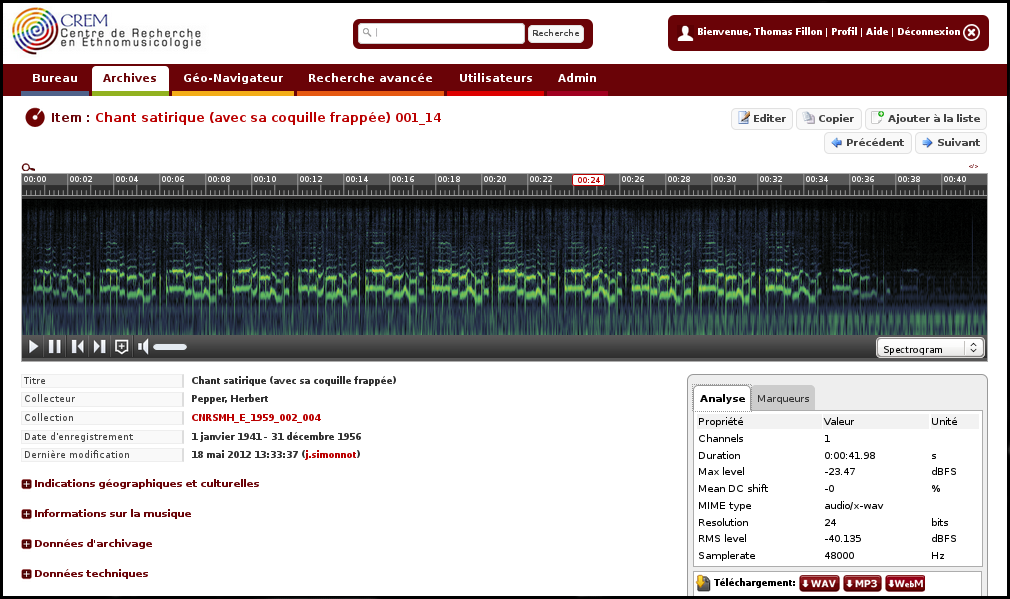
\includegraphics[width=10cm]{img/telemeta.png}
  \caption{Screenshot excerpt of the \emph{Telemeta} web interface}\label{fig:Telemeta}
\end{figure}

Telemeta is ideal for professionals who wants to easily organize, backup, archive and publish documented sound collections of audio files, CDs, digitalized vinyls and magnetic tapes over a strong database, in accordance with open web standards. 
\emph{Telemeta} architecture is flexible and can easily be adapted to particular database organization of a given sound archives. 

The main features of \emph{Telemeta} are:
\vspace{-0.1cm}
\begin{itemize}
\item \emph{Pure HTML} web user interface including high level \emph{search engine}
\item Smart \emph{workflow management} with contextual user lists, profiles and rights
  % \item RSS and JSON feed generators
  % \item XML serialized backup
\item Strong Structured Query Language (SQL) or Oracle backend
\item Model-View-Controller (MVC) architecture 
\end{itemize}
Beside database management, the audio support is mainly provided through an external component, TimeSide, which is described in Section~\ref{sec:Timeside}.

\subsection{Metadata}\label{sec:metadata}
In addition to the audio data, an efficient and dynamic management of the associated metadata is also required. %Consulting metadata provide both an exhaustive access to valuable information about the source of the data and to the related work of peer researchers. 
Dynamically handling metadata in a collaborative manner optimises the continuous process of knowledge gathering and enrichment of the materials in the database.  
%One of the major challenge is thus the standardization of audio and metadata formats with the aim of long-term preservation and usage of the different materials.
The compatibility with other systems is facilitated by the integration of the metadata standards protocols \emph{Dublin Core} and \emph{OAI-PMH} (Open Archives Initiative Protocol for Metadata Harvesting) \cite{DublinCore,OAI-PMH}.
\vspace{-0.2cm}
%Metadata provide two different kinds of information about the audio item: contextual information and annotations.
\paragraph{Contextual Information}
In ethnomusicology, contextual information could be geographic, cultural and musical. It could also store archive related information and include related materials in any multimedia format. \vspace{-0.2cm}
\paragraph{Annotations and segmentation}
Metadata also consist in temporal information such as a list of \emph{time-coded markers} associated with annotations and a list of of \emph{time-segments} associated with labels. The ontology for those labels is relevant for ethnomusicology (e.g. speech versus singing voice segment, chorus, ...).
It should be noted that annotations and segmentation can be done either by a human expert or by some automatic signal processing analysis (see Section~\ref{sec:Timeside}).


\section{TimeSide}\label{sec:Timeside}\vspace{-0.2cm}
One specificity of the Telemeta architecture is to rely on an external component, \emph{TimeSide}, that offers audio player integration together with audio signal processing analysis capabilities. Figure~\ref{fig:TimeSide_Archi} illustrates the overall architecture of \emph{TimeSide}.

\begin{figure}[htbp]
  \centering
  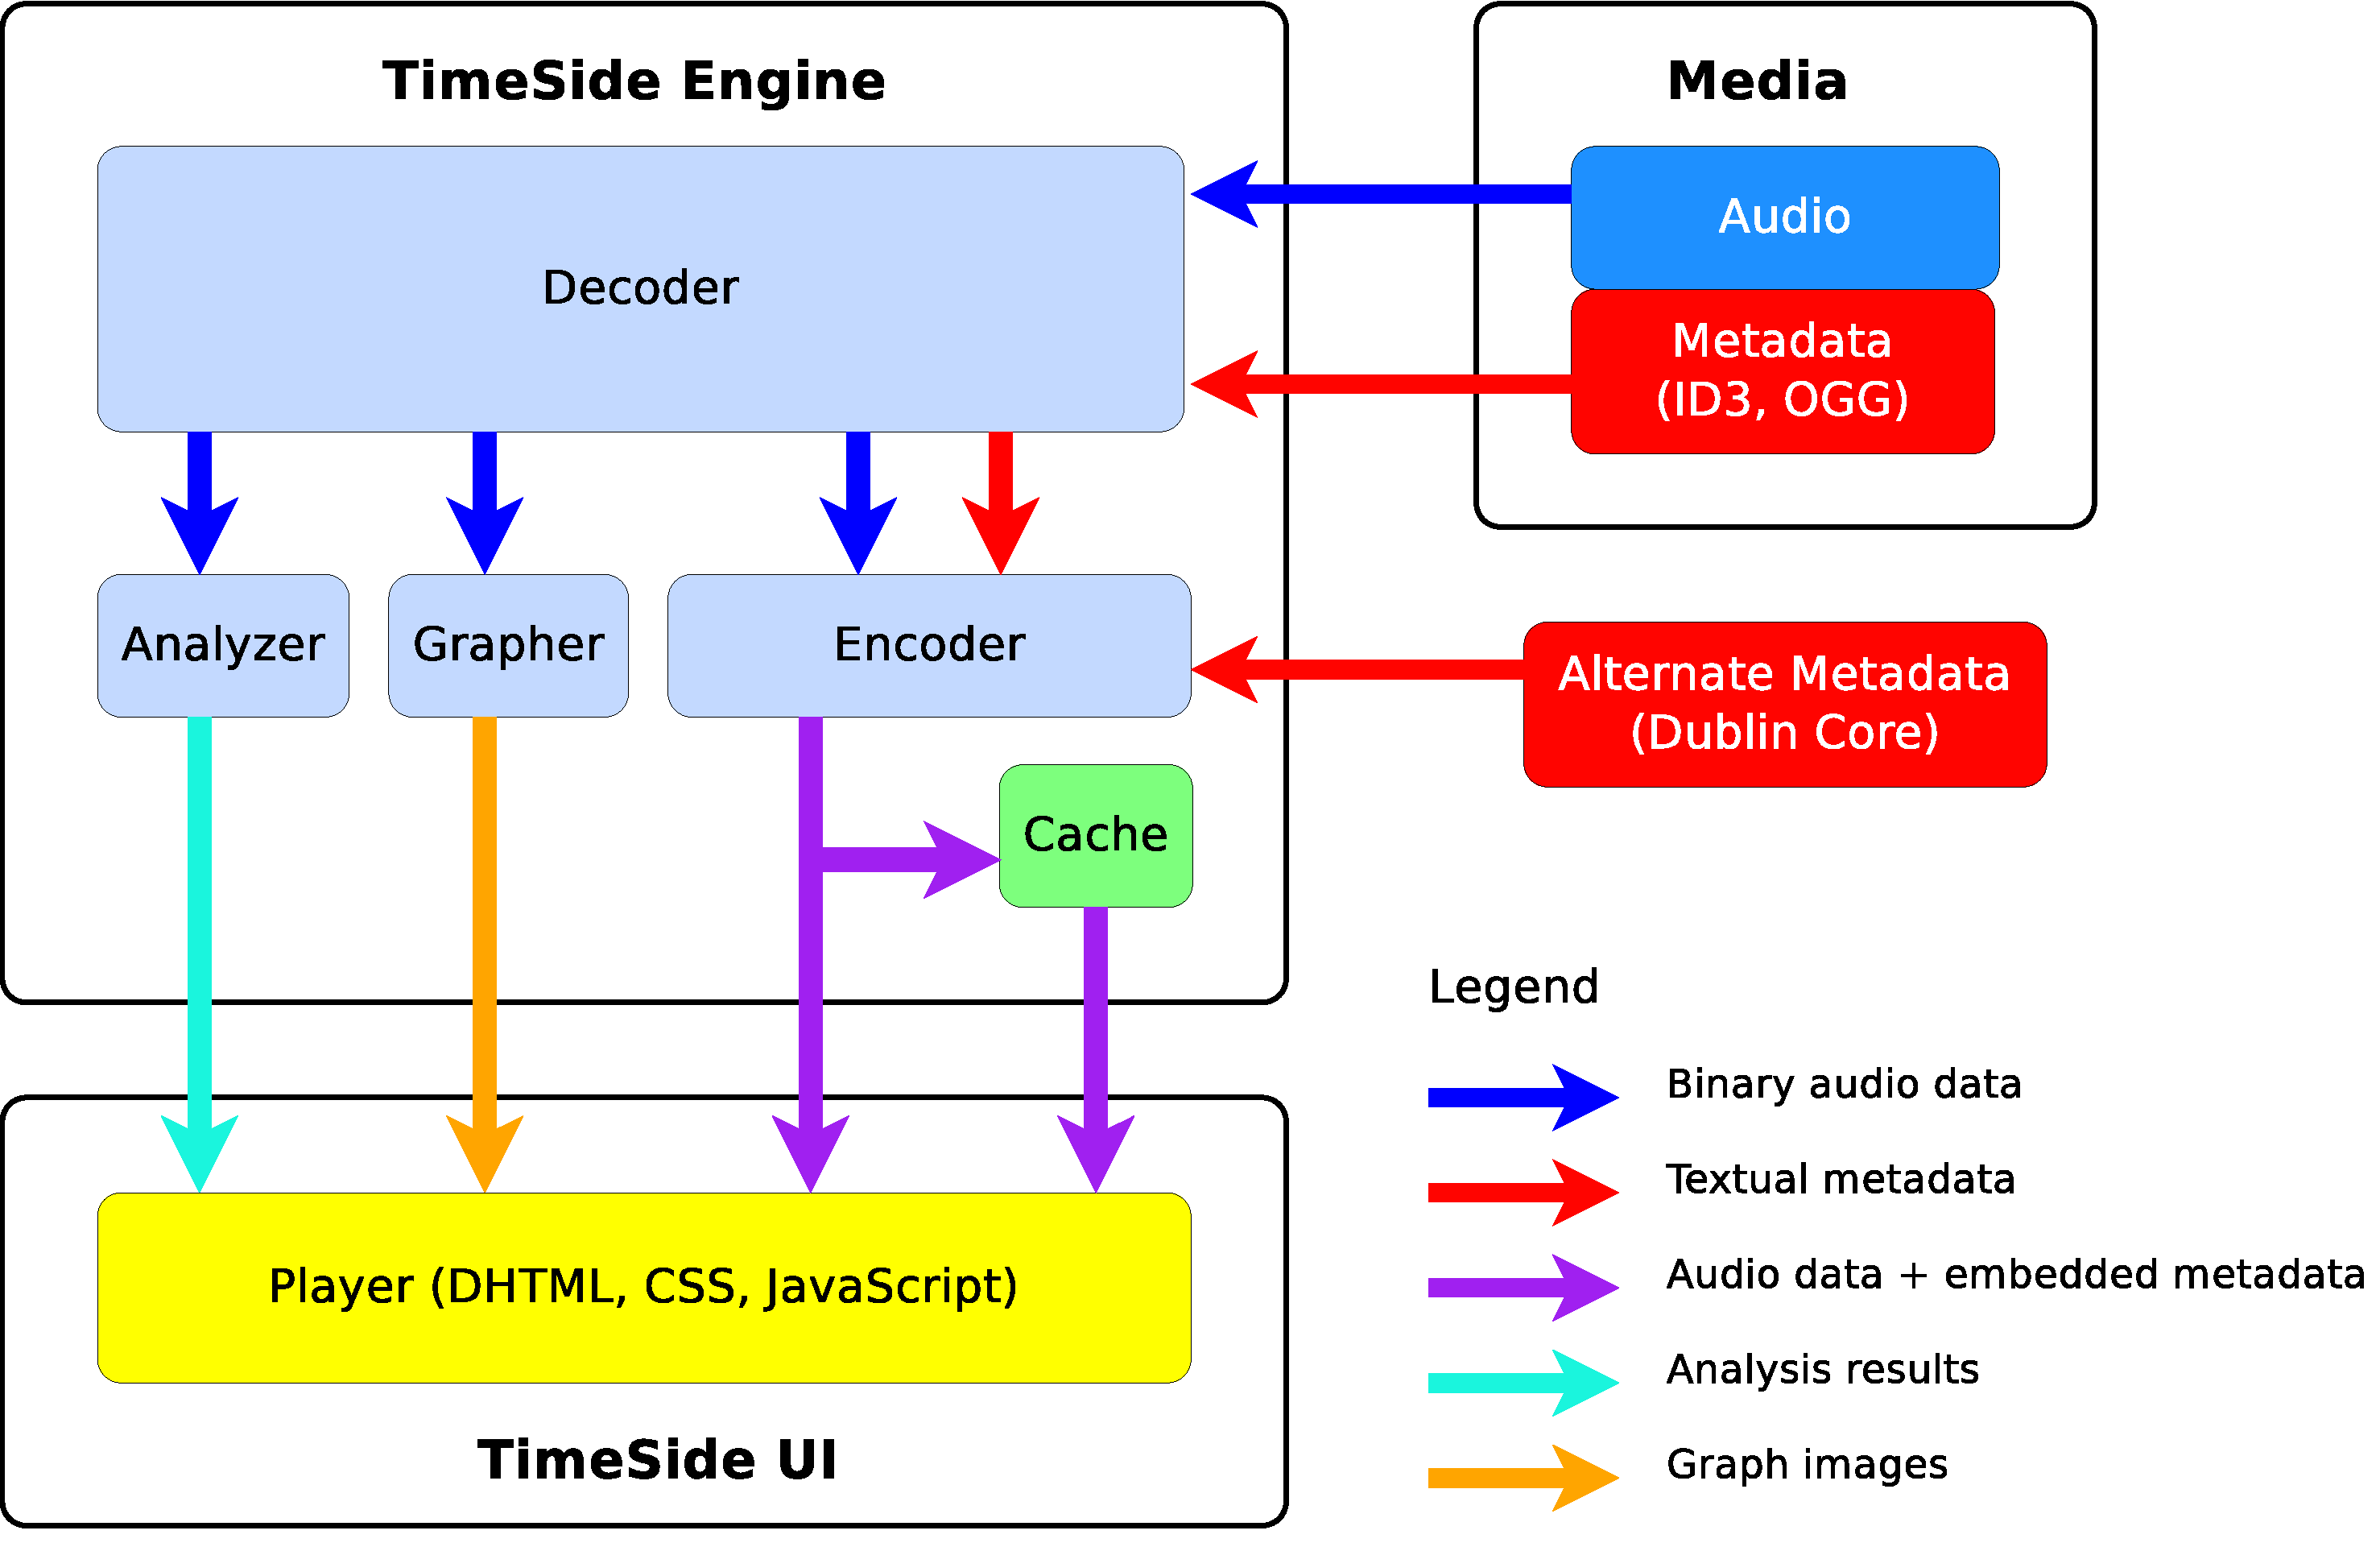
\includegraphics[width=10.5cm]{img/timeside_schema.pdf}
  \caption{TimeSide architecture (see \url{https://code.google.com/p/timeside/})}\label{fig:TimeSide_Archi}
\end{figure}

\vspace{-0.4cm}
\subsection{Audio management}
TimeSide provides the following main features:
\begin{itemize}
\item \emph{Secure archiving, editing and publishing of audio files} over
  internet.
\item Smart \emph{audio player} with enhanced visualisation (waveform, spectrogram)
\item \emph{Multi-format support}: reads all available audio and video formats  through Gstreamer, transcoding with smart streaming and caching methods% (FLAC, OGG, MP3, WAV and WebM)
  % \item \emph{Playlist management} for all users with CSV data export
\item "On the fly" \emph{audio analyzing, transcoding and metadata
    embedding} based on an easy plugin architecture
\end{itemize}
\vspace{-0.4cm}
\subsection{Audio features extraction}
TimeSide incorporates some state-of-the-art audio feature extraction libraries such as \href{http://aubio.org}{Aubio}, \href{http://yaafe.sourceforge.net}{Yaafe} and \href{http://www.vamp-plugins.org}{Vamp plugins} \cite{brossierPhD,yaafe_ISMIR2010,vamp-plugins}.
Given the extracted features, every sound item in a given collection can be automatically analyze. The results of this analysis can be displayed as a support to ethnomusicological studies.
Further works lead by the DIADEMS project will incorporate advance Music Information Retrieval methods in order to provide automatic annotation, segmentation and similarity analysis.
\vspace{-0.2cm}
\section{Conclusion - Purpose of the demonstration}\vspace{-0.1cm}
The demonstration presents the features offered by \emph{Telemeta} as detailed in Section~\ref{sec:Telemeta} in the context of ethnomusicological sound archiving \cite{telemetaCREM}. It focuses on the enhance and collaborative user-experience when accessing audio items and their associated metadata, and on the possibility for the expert user to further enrich those metadata.
Another goal of this demonstration is to present the integrated audio analysis tools described in Section~\ref{sec:Timeside}.

\vspace{-0.3cm}
\section*{Acknowledgments} \vspace{-0.2cm}
The authors would like to thank all the people that have been involved in \emph{Telemeta} specification and development or have provide useful input and feedback. 
The project has been partially funded by the French National Centre for Scientific Research (CNRS), the French Ministry of Culture and Communication, the TGE Adonis Consortium, and the Centre of Research in Ethnomusicology (CREM).

\vspace{-0.3cm}
\bibliographystyle{splncs03}
\bibliography{cmmr_2013}


\end{document}
